% Chapter Template

\chapter{Result} % Main chapter title

\label{Chapter4} % Change X to a consecutive number; for referencing this chapter elsewhere, use \ref{ChapterX}

\lhead{Chapter 4. \emph{Result}} % Change X to a consecutive number; this is for the header on each page - perhaps a shortened title

%----------------------------------------------------------------------------------------
%	SECTION 1
%----------------------------------------------------------------------------------------

\section{Maximum likelihood Classifier}

Implemented and executed Maximum Likelihood Classifier for stokes parameter with an overall accuracy = 79\%. 

\begin{table}[!htbp]
\centering
\caption{Confusion Matrix for ML Classifier}
\label{tab1}
\begin{tabular}{llll}

\hline
Class  & Forest & Non-Forest & Total Classified pixels      \\\hline
Forest         & 4,129,376 & 1,179,822 & 5,309,198 \\\hline
Non-Forest            & 786,548 & 3,736,102 & 4,522,650 \\\hline
Total ground truth pixels   & 4,915,924 & 4,915,924 & 9,831,848
\end{tabular}
\end{table}

Producer Accuracy for forest class = 83.9\%

Producer Accuracy for non-forest class = 75.9\%

User Accuracy for forest class = 77.7\%

User Accuracy for non-forest class = 82.6\%


%-----------------------------------
%	SUBSECTION 1
%-----------------------------------
\subsection{Discussion}
Upon Visually analyzing the whole image, we can observe that a huge number of pixels that were urban buildup which was not included in the groundtruth.  Figures \ref{fig61}, \ref{fig62}, \ref{fig63} below show a cropped portion of the whole image where forest area can be seen clearly.
\begin{figure} [!htbp]
\centering    
\subfigure[google earth image]{\label{fig61}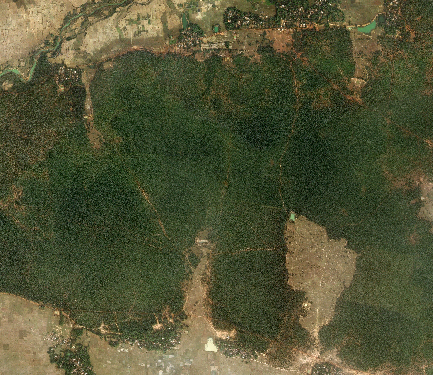
\includegraphics[width=40mm]{data3.png}}
\subfigure[RGB colour composite]{\label{fig62}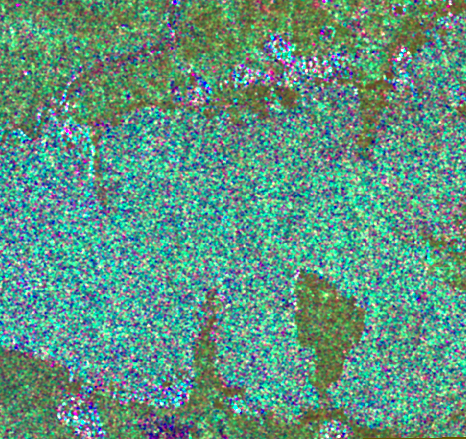
\includegraphics[width=40mm]{data2.png}}
\subfigure[classified image]{\label{fig63}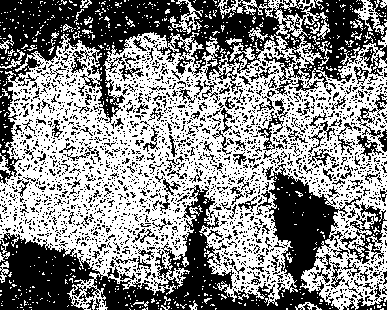
\includegraphics[width=40mm]{data4.png}}
\caption{Figures sample}
\end{figure}
The classifier required additional negative instances as ground truth to actually run and hence introduced difficulty in labelling the same. Maximum Likelihood Classifier used in the QGIS plugin tool assumes that the data pixels are normally distributed, but our data follows a complex distribution other than gaussian and hence did not give a very high accuracy . 
\begin{figure} [!htbp]
\centering    
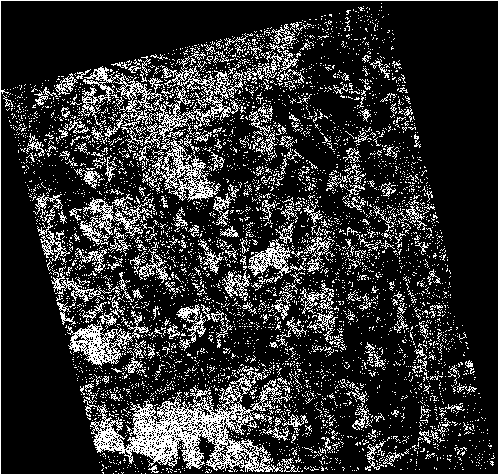
\includegraphics[width=50mm]{data8.png}
\caption{Final output image}
\end{figure}

%----------------------------------------------------------------------------------------
%	SECTION 2
%----------------------------------------------------------------------------------------

\section{One class SVM}

10-fold cross validation was done along with grid search to get the $\nu$ and $\gamma$ parameters and a producer accuracy of 99.08$\%$. for the stokes parameters feature and an accuracy of 98.81$\%$ for m-$\delta$ as feature used for classification.

\begin{table}[!htbp]
\centering
\caption{Parameter values}
\label{tab2}
\begin{tabular}{llll}

\hline
Feature  & $\nu$ & $\gamma$     \\\hline
Stokes parameters   & $9 \times 10^{-4}.$ & $3 \times 10^{-6}.$ \\\hline
m-$\delta$            & $9 \times 10^{-4}.$ & $1 \times 10^{-6}.$ \\\hline
\end{tabular}
\end{table}

%-----------------------------------
%	SUBSECTION 2
%-----------------------------------

\subsection{Discussion}
Even though, we got a good producer accuracy on the given groundtruth, when the classifier was used to predict the whole dataset, visually it was found that a large number of pixels were mispredicted as forest. 
